\documentclass[11pt,a4paper]{article}
\usepackage{babel}
\babelprovide[import,main]{english}
\usepackage[margin=2.05cm]{geometry}
\usepackage{amsmath,amssymb,graphicx,booktabs,tabularx,array,xcolor,enumitem}
\usepackage[unicode,colorlinks=true,linkcolor=teal,urlcolor=teal]{hyperref}
\hypersetup{pdftitle={Spin Network Laboratory: complete Workshop 1 description},pdfauthor={Dairon Steven Cabascango Erazo},pdfsubject={Functional progress: data structures, graph, physics, and SFML interface}}
\setlength{\parindent}{0pt}
\setlength{\emergencystretch}{2em}
\setlength{\parskip}{0.48em}
\setlist[itemize]{topsep=3pt,itemsep=2pt,leftmargin=1.5em}
\setlist[enumerate]{topsep=3pt,itemsep=2pt,leftmargin=1.8em}
\renewcommand{\arraystretch}{1.16}
\newcolumntype{Y}{>{\raggedright\arraybackslash}X}
\newcommand{\file}[1]{\texttt{\detokenize{#1}}}
\newcommand{\source}[1]{\par\vfill{\footnotesize\color{gray}Implementation sources: #1.}}
\begin{document}
\begin{center}
{\small\scshape Project Description Document}\par
\vspace{1.2cm}
{\Huge\bfseries Spin Network Laboratory}\par
\vspace{0.45cm}
{\Large Dynamic Topological Network Simulator\par in C++17 and SFML}\par
\vspace{0.8cm}
{\large\bfseries Workshop 1: Functional Progress}\par
\vspace{0.8cm}
\end{center}
\textbf{Team Members}\par
Dairon Steven Cabascango Erazo.

\textbf{Project Description}\par
Spin Network Laboratory is a computational system inspired by spin networks that enables users to construct, visualize, modify, and explore dynamic graphs. This progress submission combines custom data structures, explicit memory management, graphical interaction, and numerical integration. Vertices are stored in a custom hash table, and their connections are represented using singly linked lists. An SFML interface displays the network and allows users to edit it while an artificial force model organizes its geometry.

\textbf{Components Currently Implemented in This Submission}\par
Singly linked list; FNV-1a hash table with separate chaining and rehashing; simple undirected graph; vertex and edge models; force engine; fixed-step Velocity Verlet integrator; interaction controller; SFML rendering and basic panel; auxiliary console; automated tests; and an independent web demonstration.

\textbf{GitHub Repository Link}\par
\url{https://github.com/stevencabascango/Spin-Newtwork-of-Quantum-Gravity.git}

\textbf{Document Scope}\par
This document describes only the version preserved in the \file{Workshop 1} folder. The second submission's implementation is maintained separately. The forces are visualization tools: the program is neither a complete quantum-gravity simulation nor an implementation of the physical dynamics of LQG spin networks.

\vfill
{\small Description prepared from the local source code and its tests. Verification status as of October 10, 2026. English translation of the complete Spanish document.}
\newpage

\section{Complete Description, Purpose, and Objectives}
\subsection{Problem Addressed by the Project}
A graph represents entities and the relationships between them. When its vertices or connections are modified, the structure must preserve valid references, correct counts, and a consistent representation. Furthermore, a static drawing is insufficient for observing how geometry changes when elements are connected, moved, or removed.

The project addresses both needs: it builds a storage and editing core using custom structures and connects it to a visual simulator. Geometry evolves through artificial forces, while topology changes only through explicit user operations. Moving a node changes its position but does not create or remove connections.

\subsection{General Objective}
Develop an executable C++17 progress submission capable of storing, editing, and visualizing an undirected graph using a custom hash table and linked lists, and updating its positions through fixed-step numerical integration.

\subsection{Specific Objectives}
\begin{enumerate}
\item Implement a singly linked list supporting insertion, search, removal, clearing, and iteration.
\item Implement a hash table using FNV-1a, collision resolution by separate chaining, and controlled resizing.
\item Represent vertices through identifiers and reciprocal connections without dangling pointers between vertices.
\item Maintain simple-graph rules: no self-loops, duplicate edges, or nonexistent endpoints.
\item Incorporate elastic attraction, regularized repulsion, and damping.
\item Separate the physics step from the rendering rate using Velocity Verlet and a time accumulator.
\item Support selection, dragging, pinning, creation, connection, removal, and pausing in SFML.
\item Verify structures, dynamics, and interaction through reproducible tests.
\end{enumerate}

\subsection{Interpretation of the Model}
The term \file{QuantumVertex} belongs to the project's conceptual vocabulary: computationally, it is a labeled vertex with an artificial physical state. An edge's spin is a positive half-integer label. The model does not impose SU(2) coupling rules, quantum amplitudes, gravitational constraints, or a correspondence with the physical dynamics of quantum gravity.

The contribution of this submission is computational and educational: demonstrating that custom structures can support an editable graph and dynamic visualization. Validating this software is different from establishing a physical theory.
\source{\file{README.md}, \file{QuantumGraph.hpp}, and \file{SimulationController.hpp}}
\newpage

\section{Architecture, Objects, and Memory Management}
\subsection{Organization by Responsibility}
\begin{verbatim}
DesktopApplication -> InputController / GraphRenderer / HUD
        |
        +-- SimulationController
               +-- QuantumGraph
               |      +-- HashTable<uint64_t, QuantumVertex>
               |                    +-- QuantumVertex
               |                          +-- SinglyLinkedList<SpinEdge>
               +-- ForceEngine / VerletIntegrator / FixedStepClock
\end{verbatim}
The core and interaction logic do not need to open a window to run in the tests. SFML is used in the presentation layer: window, events, drawing, and text. This separation allows data-structure and physics failures to be evaluated independently of the graphical system.

\subsection{Vertices and Edges}
\begin{tabularx}{\linewidth}{@{}p{3.55cm}Y@{}}\toprule
Object & Stored Information \\\midrule
\file{QuantumVertex} & ID; mass and volume; current and previous position; velocity, acceleration, and force; \file{pinned} state; singly linked list of connections. \\
\file{SpinEdge} & Logical edge ID, \file{targetId}, spin, rest length, and stiffness. \\
\file{Vec2} & Two real components and elementary vector operations. \\
\file{PhysicsParameters} & Global stiffness, repulsion, damping, regularization, and fixed physics step. \\\bottomrule
\end{tabularx}
Volume is retained as a vertex attribute; it is not used to calculate forces in this version. Dynamics use mass, positions, velocities, and connection parameters. This avoids assigning a stored field a function that it does not yet perform.

\subsection{Resource Ownership}
The table owns the vertices. Each vertex owns its adjacency list. Hash-table and list nodes own their next node through \file{std::unique_ptr}; the tail pointer is a non-owning observer. Manual \file{new} and \file{delete} operations are not used to manage these nodes.

Edges contain destination IDs rather than direct pointers to the other vertex. Consequently, rehashing can rebuild storage without changing the meaning of connections. Pointers returned by \file{findVertex} are temporary observers and must not be retained across rehashing, removal, or assignment.

\subsection{Copying, Moving, and Clearing}
Lists and tables support deep copying: copying a graph duplicates its vertices and internal lists. Moving transfers structures and permits reuse of the source object. Chains are destroyed iteratively to avoid recursion proportional to their number of nodes. These capabilities prepare for the second submission's history, but do not mean that C++ history is included in Workshop 1.
\source{\file{include/Core/}, \file{include/DataStructures/}, and \file{src/Graphics/}}
\newpage

\section{Custom Singly Linked List}
\subsection{Internal Structure}
\file{SinglyLinkedList<T>} contains an owning head, a non-owning tail, and a counter. Each node stores a value of type \file{T} and a \file{unique_ptr} to the next node. The list stores each vertex's adjacencies, so traversal cost depends on that vertex's degree.
\begin{verbatim}
head -> [value | next] -> [value | next] -> [value | null]
                                                    ^
                                            tail (observer)
\end{verbatim}

\subsection{Implemented Operations}
\begin{tabularx}{\linewidth}{@{}p{4cm}Yp{1.8cm}@{}}\toprule
Operation & Behavior & Cost \\\midrule
\file{pushFront} & Inserts at the beginning; sets the tail when the list was empty. & $O(1)$ \\
\file{pushBack} & Inserts at the end without traversing the entire chain. & $O(1)$ \\
\file{find}, \file{contains} & Search by equality; search supports const or mutable access. & $O(n)$ \\
\file{remove} & Removes the first matching value. & $O(n)$ \\
\file{removeIf} & Removes by predicate; useful for finding an edge by destination. & $O(n)$ \\
\file{clear} & Dismantles the chain and leaves head and tail empty. & $O(n)$ \\
\file{size}, \file{empty} & Query the counter and empty state. & $O(1)$ \\
\file{begin}, \file{end} & Allow iteration without exposing owning nodes. & Start $O(1)$ \\\bottomrule
\end{tabularx}

\subsection{Correct Head and Tail Removal}
Removal operates on the owning link pointing to the matching node. This link may be the head or the previous node's \file{next}. The following node replaces the removed node in that link. If the tail is removed, the observer moves to its predecessor; if it was the only element, it becomes null. The counter decreases once per successful removal.

\subsection{Independent Copies and Tests}
Copying rebuilds a new chain using the source values, avoiding shared internal nodes. Assignment uses a temporary object and swapping. Moving leaves the source empty and allows new values to be inserted into it.

Tests verify insertion at both ends, successful and unsuccessful searches, head and tail removal, reinsertion after clearing, const iteration, copying, and moving. A 10\,000-element list is also constructed to check that a copy remains independent and that clearing works without manual memory deallocation.
\source{\file{SinglyLinkedList.hpp} and \file{tests/test_core.cpp}}
\newpage

\section{Hash Table: FNV-1a, Collisions, and Rehashing}
\subsection{Storage by Identifier}
\file{HashTable<uint64_t, QuantumVertex>} associates each ID with its vertex. An array of buckets starts custom chains of key--value nodes. A lookup computes the bucket and traverses its chain; it does not use \file{std::unordered_map} as a substitute for the table being evaluated.

\subsection{Implemented Hash Function}
For key bytes $b_i$, 64-bit FNV-1a is calculated as
\[
h_0=14695981039346656037,\qquad
h_{i+1}=(h_i\mathbin{\mathrm{XOR}}b_i)\,1099511628211\pmod{2^{64}}.
\]
The index is $h(k)\bmod m$, where $m$ is the number of buckets. Integer keys are encoded as little-endian bytes to obtain a result independent of the processor's byte order. The table also supports strings and an injectable alternative hash for testing.

\subsection{Collision Resolution}
Two keys with the same index are stored in the same chain but remain distinguishable by their key values. Inserting a repeated ID is rejected and does not silently overwrite the vertex. Removing an entry repairs the chain's link.
\begin{verbatim}
bucket[0] -> [key A, value] -> [key B, value] -> null
bucket[1] -> null
bucket[2] -> [key C, value] -> null
\end{verbatim}

\subsection{Load Factor and Resizing}
The load factor is $\alpha=n/m$. Before an insertion that would exceed $0.75$, the table requests a larger capacity. Rehashing rebuilds a temporary table and swaps it with the original only after all insertions are complete. Copying values during this process includes copying each vertex's adjacencies.

The final capacity may exceed a requested size that is too small to satisfy the load-factor limit. Vertex observers may become invalid: code must not depend on preserving their addresses during rehashing.

\subsection{API, Costs, and Evidence}
The API includes \file{insert}, \file{remove}, \file{find}, \file{contains}, \file{clear}, \file{size}, \file{capacity}, \file{loadFactor}, and \file{rehash}. Expected lookup cost is $O(1)$ under a suitable distribution; pathological collisions may increase it to $O(n)$.

Tests insert and retrieve 5\,000 vertices, reject duplicates, rehash to 16\,384 buckets, and remove all entries. A constant hash forces 1\,000 keys into the same bucket and verifies lookups and removals. The FNV-1a hash of \file{hello} is also checked against the expected value \file{0xa430d84680aabd0b}.
\source{\file{HashTable.hpp} and \file{tests/test_core.cpp}}
\newpage

\section{Undirected Graph and Core Components}
\subsection{Representation and Contracts}
The graph is $G=(V,E)$, simple and undirected. Vertices are indexed in the hash table, and each owns its adjacency list. Creating a connection between $a$ and $b$ inserts the records $a\to b$ and $b\to a$ with the same logical ID. The edge counter increases once, not twice.

Self-loops ($a=b$), duplicates, and nonexistent endpoints are rejected. Nonpositive mass, non-finite positions, and invalid edge parameters trigger rejection or exceptions, depending on the operation. Spin must be a positive half-integer; rest length must be positive; stiffness must be nonnegative.

\subsection{Implemented Operations}
\begin{tabularx}{\linewidth}{@{}p{4.9cm}Y@{}}\toprule
Operation & Function \\\midrule
\file{addVertex}, \file{removeVertex} & Create or remove vertices and incident connections. \\
\file{addEdge}, \file{removeEdge} & Maintain both adjacencies and the logical edge count. \\
\file{findVertex}, \file{containsVertex} & Locate vertices by ID. \\
\file{vertexCount}, \file{numberOfEdges} & Query graph sizes. \\
\file{degree}, \file{neighbors} & Query a vertex's connections. \\
\file{ids}, \file{forEachVertex} & Traverse vertices and obtain sorted IDs. \\
\file{clear}, \file{rehash} & Clear or reorganize storage. \\\bottomrule
\end{tabularx}
The original API's shorter names, \file{size}, \file{edgeCount}, and \file{contains}, are also retained. External code must not modify adjacencies directly: graph operations maintain their reciprocity.

\subsection{Removal and Consistency}
To remove a vertex, its neighbors are collected first. Each edge is removed at both endpoints, the counter decreases, and the vertex is finally removed from the hash table. No neighbor retains a connection to the removed ID. If creating an edge's second adjacency fails, the first adjacency is removed before the error is propagated.

\subsection{Complementary Metrics Already Available}
The core retains basic analysis functions and a console: vertex and edge counts, degree, connected components, and independent cycles. If $C$ is the number of connected components, a 1D graph uses $\beta_0=C$, $\beta_1=E-V+C$, and $\chi=V-E$. These functions supplement the progress submission; they are not equivalent to the second submission's analytical panel, doubly linked list, and C++ history.

\subsection{Representative Test}
A graph with 1\,000 vertices and 5\,000 edges has degree 10 at every node in the tested case. Removing vertex 0 removes its 10 connections and reduces the count to 4\,990. A copy retains the original graph; reinserting the removed ID creates an isolated vertex.
\source{\file{QuantumGraph.hpp}, \file{GraphMetrics.hpp}, and \file{tests/test_core.cpp}}
\newpage

\section{Artificial Dynamics and Parameters}
\subsection{Visualization Model}
The forces seek an understandable visual arrangement: springs for connections, pairwise repulsion, and damping to reduce oscillations. They do not change connections. Coordinates and parameters use internal simulation units; they are not presented as physical measurements in SI units.

For positions $\mathbf{x}_i$, define $\boldsymbol\Delta_{ij}=\mathbf{x}_j-\mathbf{x}_i$ and $r_{ij}=\|\boldsymbol\Delta_{ij}\|$. The implemented spring force on $i$ is
\[
\mathbf{F}^{s}_{ij}=k_{\mathrm{global}}k_{ij}(r_{ij}-L_{ij})
\frac{\boldsymbol\Delta_{ij}}{r_{ij}+\varepsilon_s}.
\]
When $r_{ij}>L_{ij}$, it attracts toward $j$; when the distance is smaller, it separates the vertices. Each logical edge is evaluated once and contributes opposite forces to its endpoints.

\subsection{Regularized Repulsion}
For a pair of distinct vertices,
\[
\mathbf{F}^{r}_{ij}=-\frac{k_r}{r_{ij}^2+\varepsilon^2}\widehat{\boldsymbol\Delta}_{ij}.
\]
Regularization initially uses $\varepsilon=5$. If two nodes coincide, a deterministic direction based on their IDs is chosen, producing separation without division by zero. The interaction is evaluated for every pair, with cost $O(V^2)$. Spin is a label: it does not directly modify forces in this progress submission.

\subsection{Damping and Mass}
The model uses $\mathbf{F}^{d}_i=-\gamma\mathbf{v}_i$ and $\mathbf{a}_i=\mathbf{F}_i/m_i$. Conservative forces are accumulated in \file{ForceEngine}; damping is applied separately in the integrator through an exponential that includes mass. A pinned node is not assigned infinite mass: \file{pinned=true} prevents its position from advancing and maintains zero velocity.

\begin{tabularx}{\linewidth}{@{}Yp{3cm}Y@{}}\toprule
Initial Parameter & Value & Role \\\midrule
Global stiffness & $2.0$ & Scales edge springs. \\
Repulsion & $12\,000$ & Prevents excessive clustering. \\
Damping & $2.0$ & Reduces velocities and oscillations. \\
Regularization & $5.0$ & Bounds repulsion at small distances. \\
Preset rest length & $90$ & Rest length per edge. \\
Preset mass & $1.0$ & Artificial inertial response. \\\bottomrule
\end{tabularx}
For an internal dimensional interpretation, effective stiffness has dimension $M/T^2$, repulsion has dimension $ML^3/T^2$, and damping has dimension $M/T$. These numbers are graphical-model parameters, not gravitational constants.
\source{\file{ForceEngine.hpp}, \file{PhysicsParameters.hpp}, and \file{QuantumVertex.hpp}}
\newpage

\section{Velocity Verlet and Fixed-Step Updates}
\subsection{Conservative Algorithm}
Velocity Verlet divides the velocity impulse into two half-steps. Forces are first calculated at the current position; the position is then advanced, and forces are recalculated:
\begin{align*}
\mathbf{v}_{n+1/2}&=\mathbf{v}_n+\tfrac{\Delta t}{2}\mathbf{a}_n,\\
\mathbf{x}_{n+1}&=\mathbf{x}_n+\Delta t\,\mathbf{v}_{n+1/2},\\
\mathbf{a}_{n+1}&=\mathbf{F}(\mathbf{x}_{n+1})/m,\\
\mathbf{v}_{n+1}&=\mathbf{v}_{n+1/2}+\tfrac{\Delta t}{2}\mathbf{a}_{n+1}.
\end{align*}
The implemented version incorporates damping through symmetric operator splitting. With $d=\exp[-\gamma\Delta t/(2m)]$, it performs
\[
\mathbf{v}_{1/2}=d\mathbf{v}_n+\tfrac{\Delta t}{2}\mathbf{a}_n,
\qquad
\mathbf{v}_{n+1}=d\bigl(\mathbf{v}_{1/2}+\tfrac{\Delta t}{2}\mathbf{a}_{n+1}\bigr).
\]
Position advances using $\mathbf{v}_{1/2}$. This avoids treating velocity-dependent damping as a force that depends only on position.

\subsection{Physics Clock Independent of FPS}
The fixed step is $\Delta t=1/120$ s. \file{FixedStepClock} accumulates elapsed time between frames and executes complete steps. At 60 FPS, two physics steps are normally performed per frame; the variable frame duration is not used directly as the integration step.

Pausing resets the accumulator so that paused time is not recovered. A long suspension is limited to $0.1$ s of catch-up, at most 12 steps. This policy deliberately discards time after prolonged stalls; FPS equivalence is checked under conditions without such stalls.

\subsection{Pinning, Dragging, and Checks}
A pinned or dragged vertex maintains its position during physics updates and has zero velocity. Dragging preserves the offset between the node's center and the grab point, preventing an initial jump. Previous position and acceleration are updated as part of the numerical state.

Tests compare results after one second at 30, 60, and 144 FPS using a positional tolerance of $10^{-8}$. An undamped oscillator maintains relative energy error below $0.1\%$ after 1\,200 steps; the damped test confirms dissipation. A free mass follows the expected decay $v(t)=v(0)e^{-\gamma t/m}$. These are checks of the executed cases, not a universal guarantee of stability for every parameter or graph.
\source{\file{VerletIntegrator.hpp} and \file{tests/test_physics.cpp}}
\newpage

\section{SFML Interface, Controls, and Complementary Demo}
\subsection{Implemented Presentation}
\file{GraphRenderer} draws edges as segments, vertices as circles, and IDs beside the nodes. \file{HUD} displays tools, counts, pause status, parameters, and FPS. \file{InputController} translates events and screen coordinates into graph actions; the camera frames the graph without changing its geometry.

\begin{tabularx}{\linewidth}{@{}Yp{6.9cm}@{}}\toprule
Action & Workshop 1 Control \\\midrule
Select / drag & Left mouse button; Select tool or \file{S}. \\
Add a vertex & Add button and click; \file{A} on the canvas. \\
Create an edge & \file{C} or Connect tool; source and destination. \\
Remove selection / element under pointer & \file{Delete} / \file{D} and click. \\
Pause / pinning / positions & \file{Space} / \file{P} / \file{R}. \\
Repulsion / stiffness / damping & Up/down arrows; brackets; comma/period. \\
Initial network / 100-node network & \file{1} / \file{2}. \\
Frame network / close & \file{F} / \file{Esc}. \\\bottomrule
\end{tabularx}
The initial network has 20 nodes and 43 edges; the 100-node configuration has 261 edges. The visual interaction limit is 500 vertices, independent of hash-table capacity. Resetting positions preserves topology and pinned states.

\subsection{Independent Web Demo}
\begin{center}
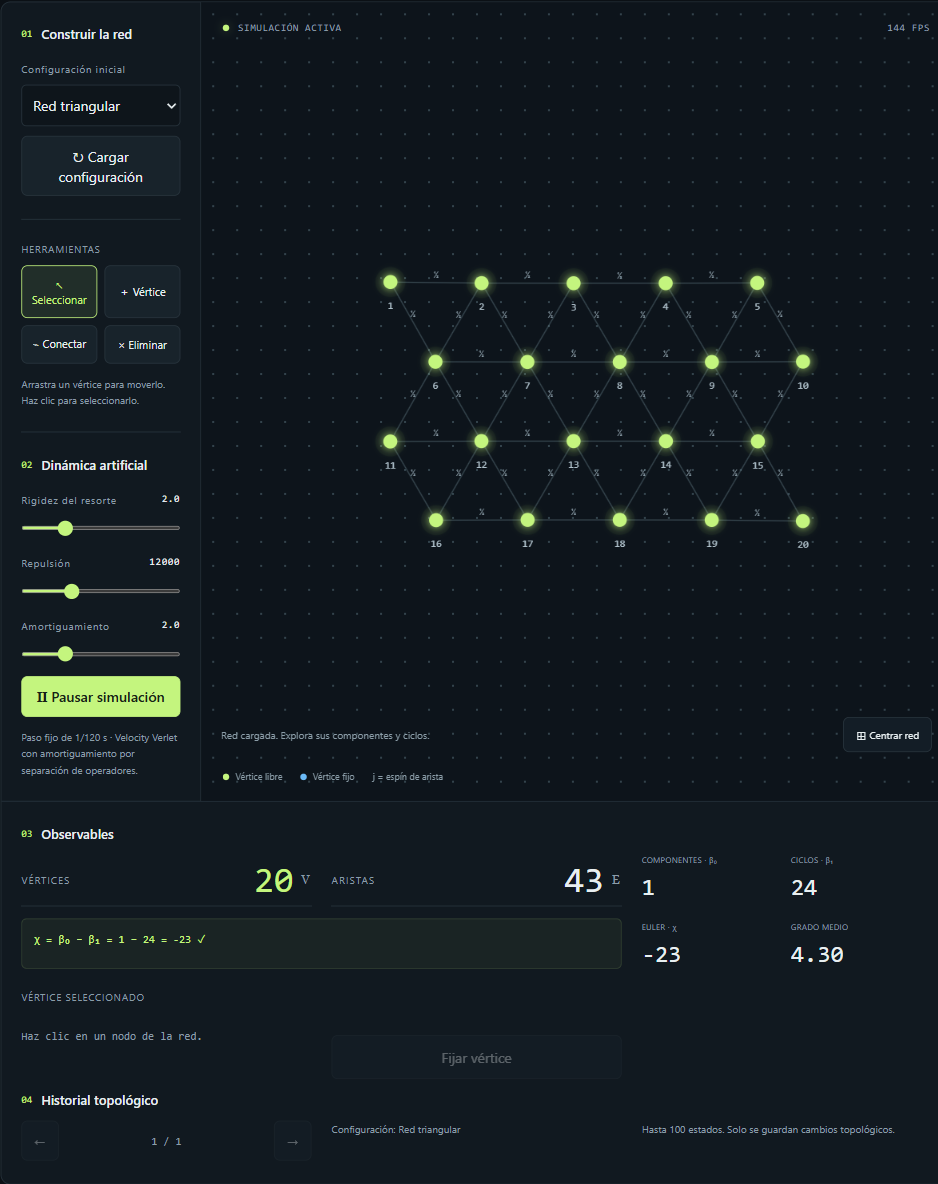
\includegraphics[width=0.86\linewidth,height=6.1cm,keepaspectratio]{../screenshots/workshop1-web.png}\\[-1mm]
{\footnotesize Actual progress-demo screenshot in Brave; not an SFML screenshot. Original Spanish-language interface retained as recorded evidence.}
\end{center}
The \file{site/dist/index.html} page is an independent JavaScript program and can be opened without a server. It displays editing, forces, and metrics; its web history is complementary and does not establish that a doubly linked list or C++ history exists in Workshop 1. Changes are lost when the page is reloaded.

The native application is implemented and compiled, but X11 display access was blocked in the restricted environment. Therefore, this document distinguishes controls tested in the controller from a full visual validation of the SFML window, which remains pending.
\source{\file{src/Graphics/}, \file{SimulationController.hpp}, and the local web-demo screenshot}
\newpage

\section{Tests, Results, and Computational Complexity}
\subsection{Evidence for the Progress Submission}
Workshop 1 has three suites: \file{test_core}, \file{test_physics}, and \file{test_interaction}. Their binaries were rerun on October 10, 2026, and completed successfully. Results are supported by assertions in their source files, not replaced by visual inspection of the code.

\begin{tabularx}{\linewidth}{@{}p{3.6cm}Y@{}}\toprule
Verified Case & Result \\\midrule
Custom hash table & Insertion/retrieval of 5\,000 vertices; duplicates rejected; rehashing and complete removal. \\
Collisions & 1\,000 keys forced into one bucket; lookups and removal at the ends and interior. \\
Singly linked list & Operations, copying/moving, and a 10\,000-element chain. \\
Graph & 1\,000 vertices, 5\,000 edges, and incident-edge removal. \\
Numerical stability & 100 nodes and 261 edges over 7\,200 steps: 60 simulated seconds, finite states. \\
FPS independence & Matching states in the tested case at 30/60/144 FPS. \\
Interaction & Creation, connection, self-loop/duplicate rejection, dragging, pinning, pausing, and removal. \\\bottomrule
\end{tabularx}

\subsection{Algorithm Costs}
\begin{tabularx}{\linewidth}{@{}Yp{6.8cm}@{}}\toprule
Operation & Cost / Scope \\\midrule
List: insert at front/end & $O(1)$. Search/removal: $O(n)$. \\
Hash lookup & Expected $O(1)$; $O(V)$ in pathological chains. \\
Rehashing / graph copying & Expected $O(V+E)$; pathological collisions can increase rebuilding cost. \\
Forces / Verlet step & Expected $O(V^2+E)$; two force evaluations. \\
Drawing & Expected $O(V+E)$. \\
Sorted IDs & $O(V\log V)$; auxiliary to position reset and traversal. \\\bottomrule
\end{tabularx}
These costs assume reasonably distributed hash chains. Copying a vertex includes its adjacencies. Stability with 100 nodes does not justify promising performance for millions of elements.

\subsection{Pending Checks}
Progress records report successful ASan/UBSan checks with \file{detect_leaks=0}. LeakSanitizer did not work under ptrace: verified absence of leaks is not claimed. Neither the SFML window in the sandbox nor Windows/Code::Blocks compilation was verified. The \file{--smoke-test} and manual demonstration procedure are prepared for a display-enabled desktop.
\source{\file{tests/test_core.cpp}, \file{test_physics.cpp}, \file{test_interaction.cpp}, and \file{docs/validation.md}}
\newpage

\begingroup\small
\section{Files, Execution, and Repository Link}
\subsection{Workshop 1 Deliverable}
\begin{verbatim}
Workshop 1/
  main.cpp                  SpinNetworkLaboratory.cbp
  CMakeLists.txt            README.md / ENTREGA.txt
  include/                  src/
  tests/                    assets/fonts/
  docs/architecture.md      docs/validation.md
  docs/report/              site/dist/
  tools/                    bin/ / .deps/sfml/
\end{verbatim}
The folder preserves the progress submission independently. Source files, resources, build configuration, and tests are included. The supplied local SDK and binaries target Linux x86\_64; they are not Windows executables.

\subsection{Reproducible Build and Execution}
From the Workshop 1 folder, with compatible GCC C++17 and SFML 2.6:
\begin{verbatim}
./tools/build.sh
./bin/spin_network
./tools/build.sh --core-only
./bin/spin_network --smoke-test
\end{verbatim}
The \file{--core-only} mode tests structures, physics, and interaction without SFML. CMake uses \file{cmake -S . -B build}, \file{cmake --build build}, and \file{ctest --test-dir build --output-on-failure}. When using the local SDK, its prefix must be supplied during configuration.

On Windows, open \file{SpinNetworkLaboratory.cbp} in Code::Blocks, configure an SFML 2.6 MinGW SDK compatible with the compiler, link graphics/window/system, and place the DLLs and resources alongside the program. Integration instructions are supported by the official SFML documentation \cite{sfml}.

\subsection{Provided Repository}
\url{https://github.com/stevencabascango/Spin-Newtwork-of-Quantum-Gravity.git}

The link is reproduced exactly as supplied by the team member. The described content and tests concern the local Workshop 1 copy; this document does not certify that the remote repository has the same state. The second submission includes a doubly linked list, C++ history, undo/redo, the final analytical panel, and refinement; these features are not attributed to the progress submission described here.

\subsection{References and Document Preparation}
{\footnotesize
\begin{thebibliography}{9}
\bibitem{sfml} SFML. \emph{SFML and Linux}, official documentation, version 2.6. \url{https://www.sfml-dev.org/tutorials/2.6/getting-started/linux/}. Supports build and linking configuration.
\bibitem{local} Local source code of \emph{Spin Network Laboratory, Workshop 1}: \file{include/}, \file{src/}, \file{tests/}, \file{README.md}, and \file{docs/validation.md}. Basis for the description and results.
\bibitem{skills} Kassis, T.; Agarwal, V.; He, Y.; Patel, D.; Brueckner, A. M. (2026). \emph{Scientific Agent Skills: A Library of Procedural Knowledge for Research Agents}. \url{https://doi.org/10.48550/arXiv.2609.00065}. Methodological tool for assisted preparation; not evidence for the simulator's results.
\end{thebibliography}}
\endgroup
\end{document}
